\documentclass[a4paper,10pt]{article}

\usepackage[utf8]{inputenc}
\usepackage[spanish]{babel}

\usepackage{graphicx}
\usepackage{float}
\usepackage{amsmath,amssymb}
\usepackage{subcaption}


\author{Jonathan Teran - LU: 643/18}
\title{Redes Neuronales - Trabajo Práctico 2}
\date{}

\begin{document}
\maketitle

\section{Introducción}

En este trabajo se presentarán dos modelos de aprendizaje hebbiano no
supervisado, que se utilizarán para reducir la dimensión de unos documentos de
entrada. Estos difieren en la regla que se utiliza para actualizar los pesos
en cada iteración del algoritmo:

\begin{itemize}
	\item Regla de Oja,
	\item Regla de Sanger
\end{itemize}

Se explicará brevemente de que consiste cada regla, cómo solucionan nuestro
problema, y que diferencias presentan estas soluciones.

\section{Reducción de dimensión por PCA}

El problema a resolver consiste en, dada una instancia de dimensión $N$,
encontrar una representación de menor dimensión $M \ll N$. Cada una de estas
instancias tiene asignada como principal 1 de 9 categorías posibles, la cual
depende del vector que representa a cada instancia.

Una manera de lograr esta reducción es estudiando las componentes principales
de las instancias. Debido a que las proyecciones de las instancias sobre estas
componentes tienen varianza máxima, conservan la mayor cantidad de
información y son ideales para utilizarlas como ejes sobre las que
representaremos las instancias en $M$ dimensiones. En este problema en
particular, haremos una reducción a $M=9$ dimensiones, por lo que
necesitaremos llevar estas instancias al sub-espacio generado por las primeras
9 componentes principales.

La implementación de estos algoritmos utiliza como criterio de parada una
medida de la ortogonalidad de los $M$ vectores de la matriz de pesos $W$. Sea
$o(W)$ la medida de esta ortogonalidad, calculada como:

\[ o(W) = sum(abs(W^TW - I))/2 \]

, donde $abs(M)$ es la matriz resultante de obtener el valor absoluto de cada
elemento, $sum(M)$ obtiene la suma de todos los elementos de la matriz, e $I$
es la matriz identidad de $\mathbb{R}^{M \times M}$. $W^TW$ calcula el producto interno
entre cada par de vectores de $W$, de modo que cuando todos sean ortogonales
entre sí, el resultado de $W^TW$ será la matriz identidad $I$, y $o(W)$ será
igual a 0. Nuestro criterio de parada será $ort(W) < 0.05$.

Para que esta convergencia de la matriz de pesos sea lo más amena posible, se
implementó un \textit{learning rate} dinámico. En una primera implementación
se decidió actualizar el mismo en cada época $t$ como una fracción $\tfrac{1}{t}$ del $lr$
inicial, $lr_0$. Sin embargo, para la implementación con la regla de Sanger, el $lr$
efectivo para las últimas épocas terminó siendo muy chico y la velocidad de
convergencia hacia la matriz $W$ objetivo muy lenta. Es por esto que se
decidió utilizar otro contador, $lr_\alpha$, con valor inicial 1, que
se incremente con un $\Delta lr = 0.6 < 1$. En cada época $t$, el valor de $lr$ se
calcula como $lr_t = \tfrac{lr_0 }{lr_\alpha}$, y se actualiza $lr_\alpha := lr_\alpha
+ \Delta lr_\alpha$.

\subsection{Algoritmo implementado con regla de Oja}

La regla de Oja actualiza los pesos de forma tal que estos convergen a
vectores ortogonales entre sí, que generan el mismo sub-espacio generado por
las primeras $M$ componentes principales.

\begin{figure}[H]
	\centering
	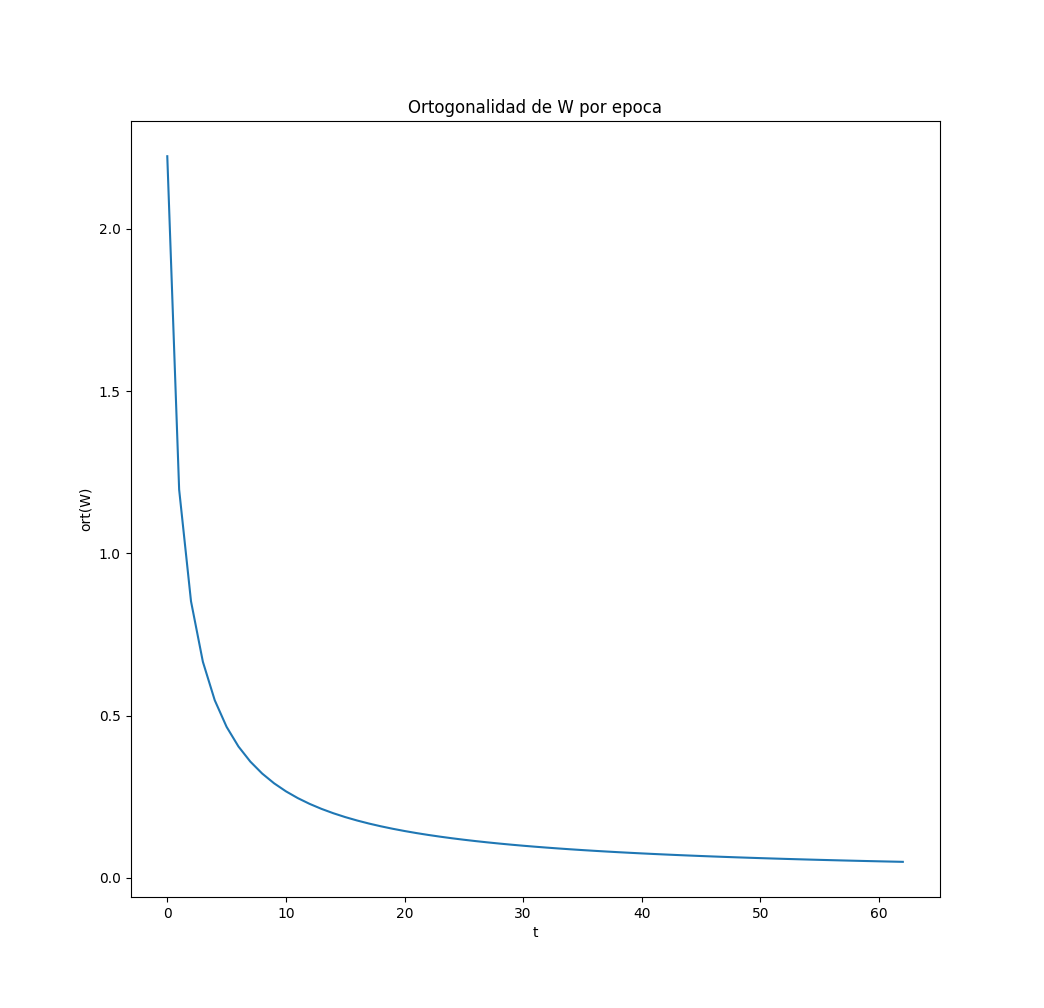
\includegraphics[width=.7\textwidth]{imgs/oja-ortw_vs_epocas.png}
	\caption{Regla de Oja: $ort(W)$ vs. época}
	\label{fig:oja-ortw_vs_epocas}
\end{figure}

En la Figura \ref{fig:oja-ortw_vs_epocas} podemos observar los valores que
toma el valor de $ort(W)$ en cada época. Más adelante veremos que esta regla
tiene una convergencia mucho más rápida que la regla de Sanger.

\begin{figure}[H]
	\begin{subfigure}{.5\textwidth}
		\centering
		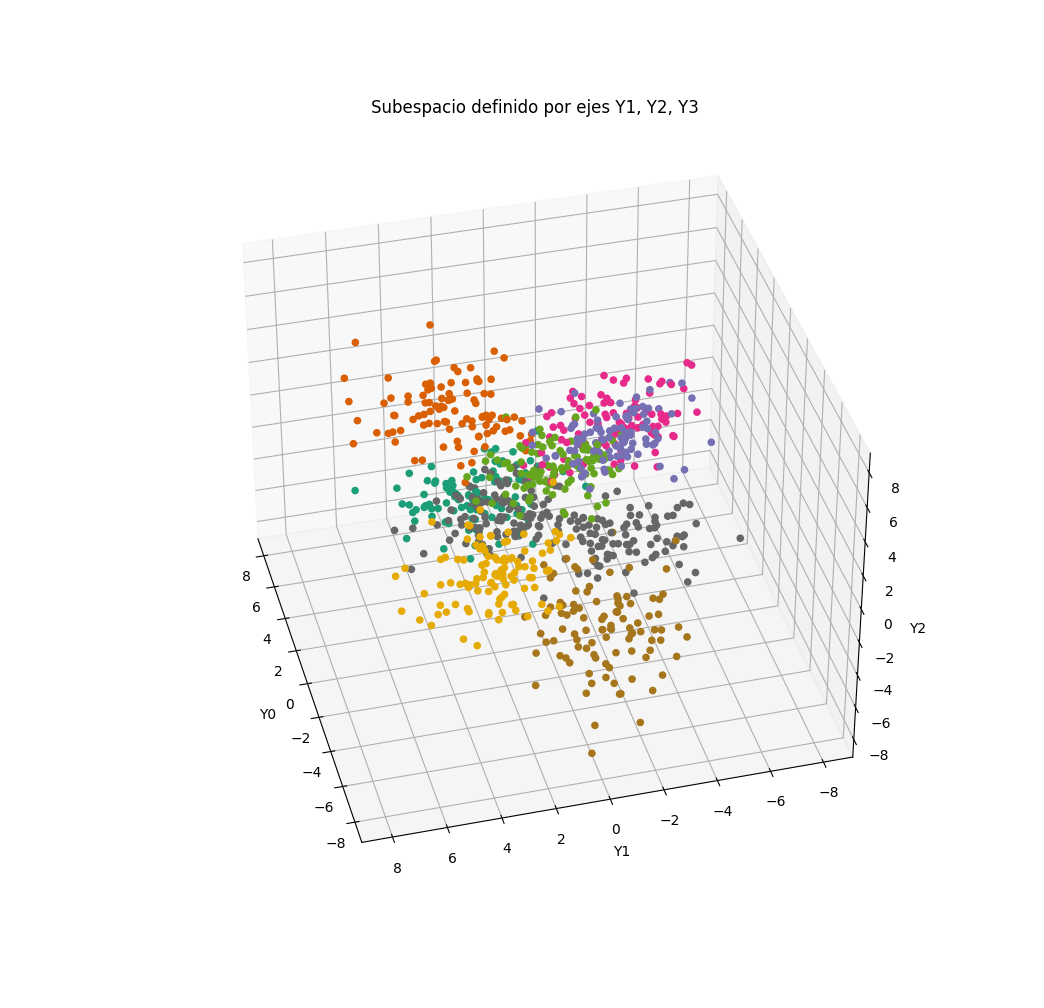
\includegraphics[width=\textwidth]{imgs/oja-subespacio-y1_y2_y3.png}
		\caption{Ejes $Y_1$, $Y_2$, $Y_3$}
		\label{fig:oja-1er_subesp}
	\end{subfigure}%
	\begin{subfigure}{.5\textwidth}
		\centering
		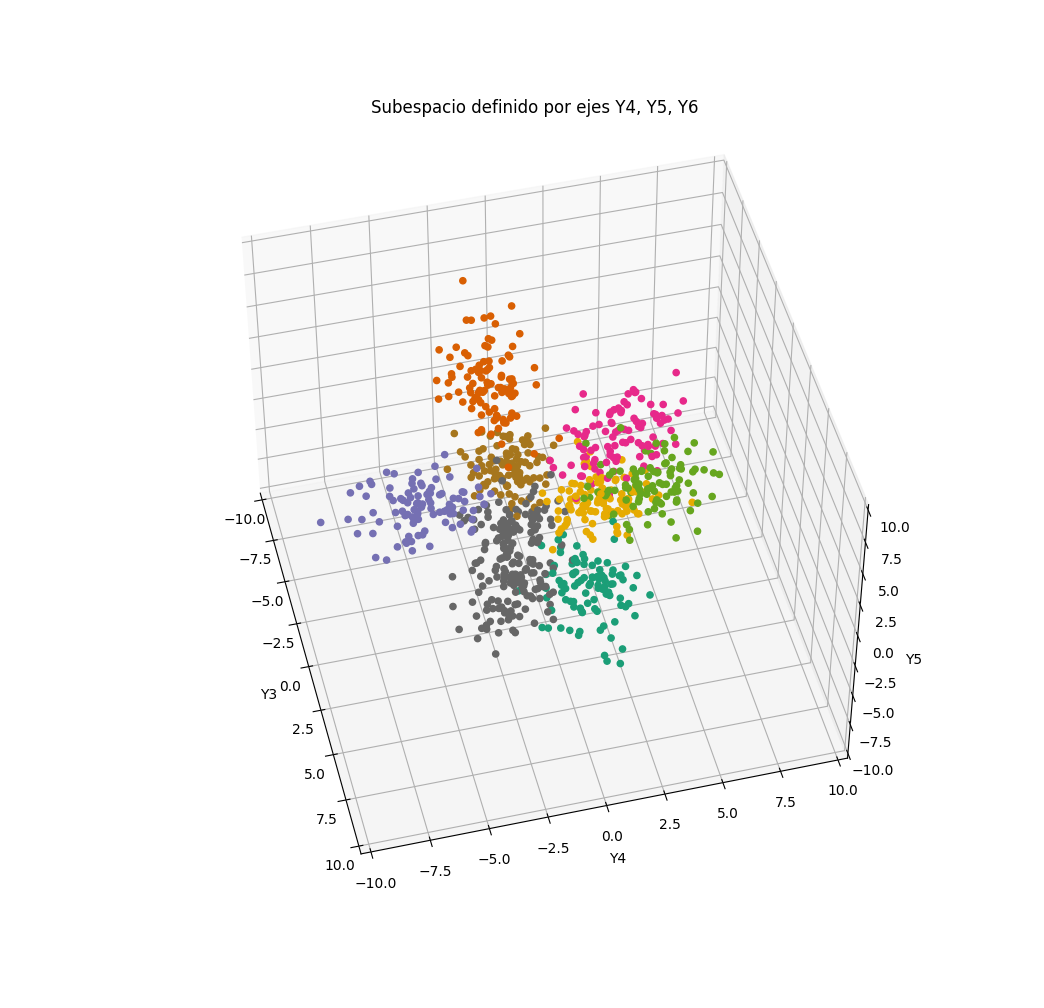
\includegraphics[width=\textwidth]{imgs/oja-subespacio-y4_y5_y6.png}
		\caption{Ejes $Y_4$, $Y_5$, $Y_6$}
		\label{fig:oja-2er_subesp}
	\end{subfigure}
	\begin{center}
		\begin{subfigure}{.5\textwidth}
			\centering
			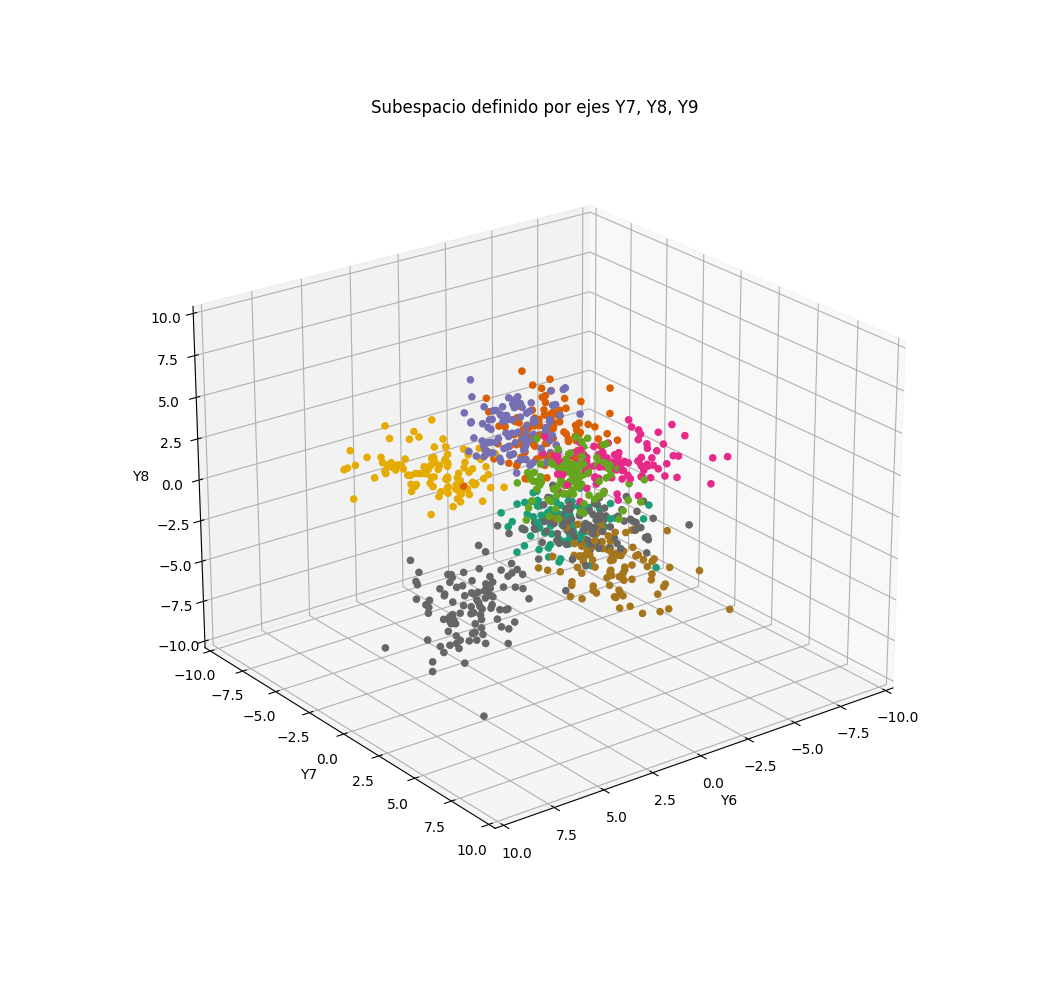
\includegraphics[width=\textwidth]{imgs/oja-subespacio-y7_y8_y9.png}
			\caption{Ejes $Y_7$, $Y_8$, $Y_9$}
			\label{fig:oja-3er_subesp}
		\end{subfigure}
	\end{center}

	\caption{Regla de Oja: Subespacios generados por cada eje}
	\label{fig:oja-subespacios}
\end{figure}

En la Figura \ref{fig:oja-subespacios} se encuentran 3 gráficos que
representan las instancias de entrada como proyecciones en los 9 vectores
encontrados por el algoritmo, y cada vértice tiene asignado un color
correspondiente a la categoría principal de cada instancia.

Cada una se tomo desde un ángulo tal que se presente la menor cantidad de
superposiciones entre las categorías, pero como se puede observar, esta no fue
tarea fácil ni se completo con éxito.

\subsection{Algoritmo implementado con regla de Sanger}

La regla de Sanger nos asegura algo más que la de Oja. Los vectores
encontrados son las primeras $M$ componentes principales de las instancias de
entrada.

\begin{figure}[H]
	\centering
	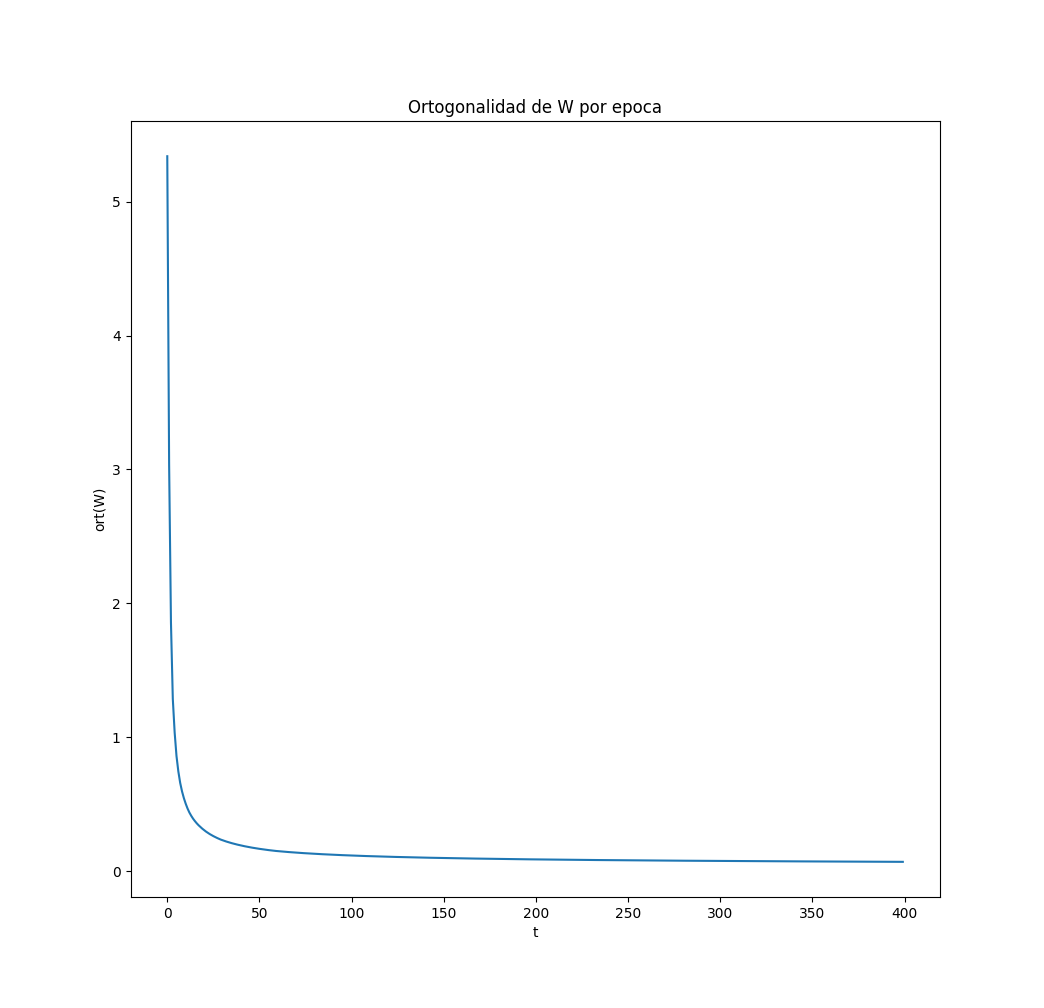
\includegraphics[width=.7\textwidth]{imgs/sanger-ortw_vs_epocas.png}
	\caption{Regla de Sanger: $ort(W)$ vs. época}
	\label{fig:sanger-ortw_vs_epocas}
\end{figure}

Esta nueva garantía ciertamente incrementa el tiempo de ejecución necesario
para encontrar los vectores o componentes principales (C.P.). Mientras que con la
regla de Oja, solo necesitábamos 9 vectores ortogonales en el subespacio de
las primeras 9 C.P., ahora necesitamos estas últimas. Se puede observer en la
Figura \ref{fig:sanger-ortw_vs_epocas} que incluso después de 400 épocas, no
se logro llegar al valor de ortogonalidad que definimos como condición de
parada.

Es de esperarse entonces, que las proyecciones sobre estos vectores
den lugar a una división entre las categorías aún más pronunciada, puesto que
la proyección sobre estos vectores presentan varianza máxima.

\begin{figure}[H]
	\begin{subfigure}{.5\textwidth}
		\centering
		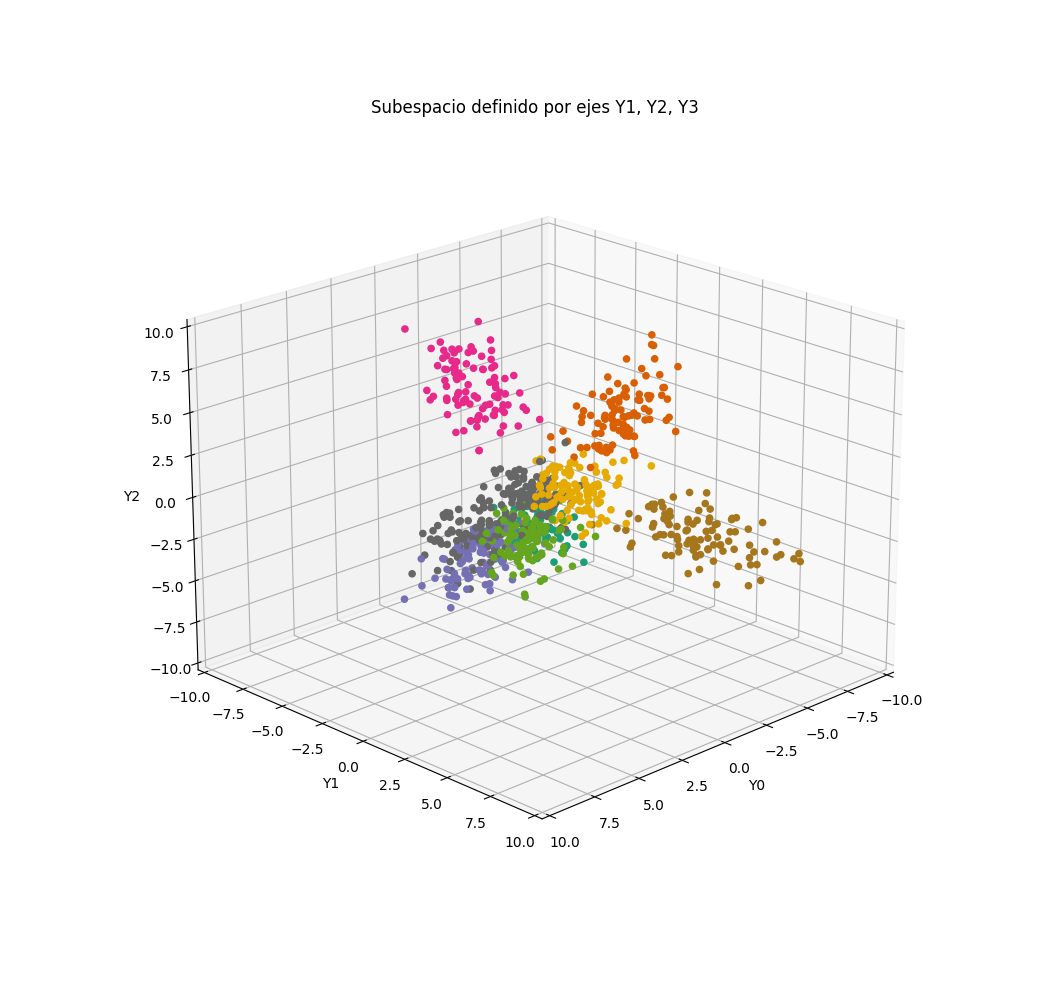
\includegraphics[width=\textwidth]{imgs/sanger-subespacio-y1_y2_y3.png}
		\caption{Ejes $Y_1$, $Y_2$, $Y_3$}
		\label{fig:sanger-1er_subesp}
	\end{subfigure}%
	\begin{subfigure}{.5\textwidth}
		\centering
		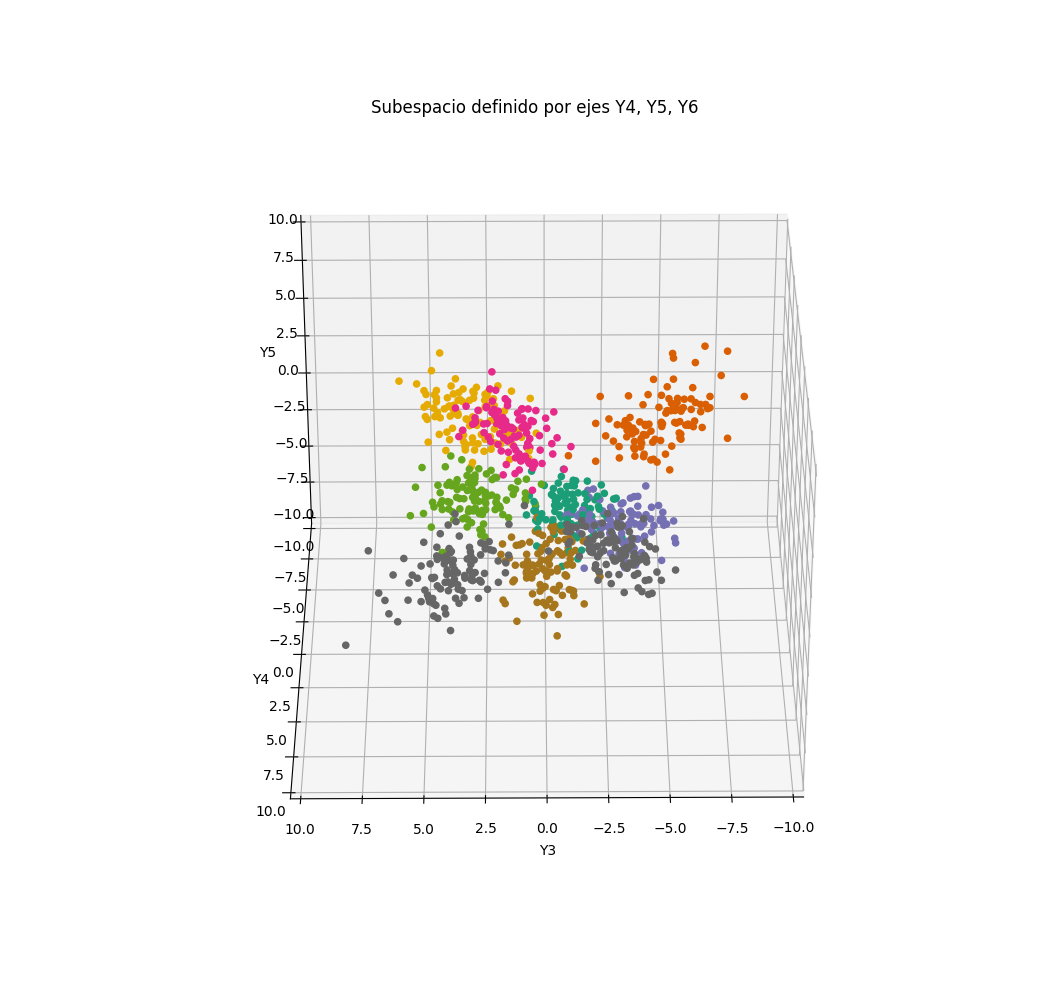
\includegraphics[width=\textwidth]{imgs/sanger-subespacio-y4_y5_y6.png}
		\caption{Ejes $Y_4$, $Y_5$, $Y_6$}
		\label{fig:sanger-2er_subesp}
	\end{subfigure}
	\begin{center}
		\begin{subfigure}{.5\textwidth}
			\centering
			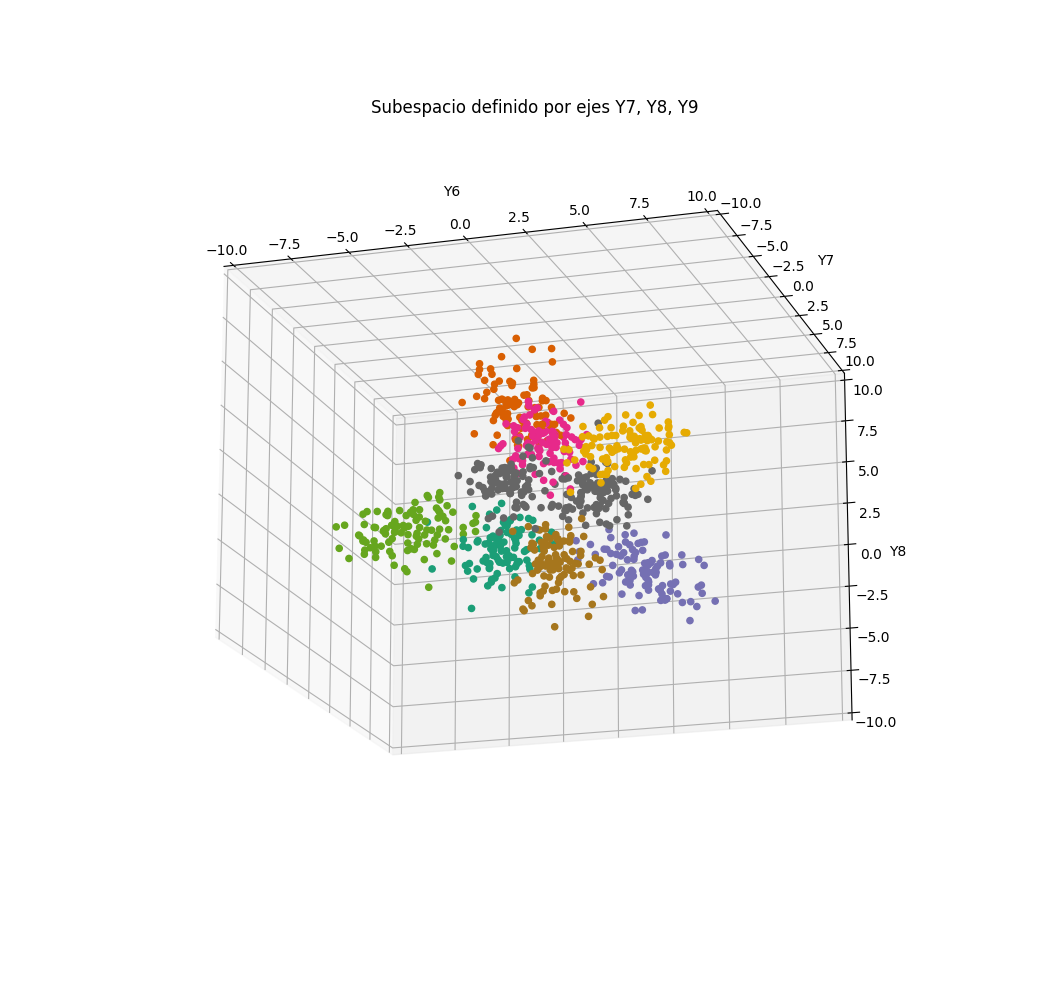
\includegraphics[width=\textwidth]{imgs/sanger-subespacio-y7_y8_y9.png}
			\caption{Ejes $Y_7$, $Y_8$, $Y_9$}
			\label{fig:sanger-3er_subesp}
		\end{subfigure}
	\end{center}

	\caption{Regla de Sanger: Subespacios generados por cada eje}
	\label{fig:sanger-subespacios}
\end{figure}

Nuevamente cada vértice tiene asignado un color correspondiente con su
categoría principal. Si compara estas proyecciones con las de a Figura
\ref{fig:oja-subespacios}, notaremos que ahora las superposiciones son
mínimas. Si bien la Figura \ref{fig:sanger-1er_subesp} presenta
superposiciones entre las categorías, también es la que presenta mayor
separación entre categorías, tomando la rosa y la marrón como ejemplos. En las
siguientes podemos distinguir claramente las 9 categorías (2 de las cuales
lamentablemente tienen colores oscuros muy similares, pero se pueden diferenciar
en la Figura \ref{fig:sanger-2er_subesp}, y están ligeramente separadas en la
Figura \ref{fig:sanger-3er_subesp})

\section{Conclusiones}

Comparando los gráficos de ortogonalidad por época, y las proyecciones sobre
los vectores obtenidos de cada regla, es fácil notar cuales son las fortalezas
y debilidades de cada una. La regla de Oja ofrece una convergencia a una
solución mucho más rápida que la de Sanger. Sin embargo la solución obtenida
por Sanger produce proyecciones que preservan más información de las
instancias de entrada que las de Oja.

La elección de una regla por sobre la otra ciertamente depende de la
aplicación que se le quiera dar a los resultados. Podríamos aplicar la regla
de Oja a algunas capas en una red de aprendizaje supervisado que utilice un
método de aprendizaje costoso en tiempo de ejecución, como lo es
Backpropagation. Por otro lado la de Sanger se podría utilizar para compresión
de información que se persista en algún tipo de memoria, ya que en estos casos
se puede justificar un tiempo de ejecución mayor.
\end{document}
